

\documentclass[11pt,a4paper]{article}
\usepackage[hyperref]{acl2018}
\usepackage{times}
\usepackage{latexsym}
\newcommand\tab[1][1cm]{\hspace*{#1}}
\usepackage{url}
\usepackage{graphicx}
\usepackage{enumitem}
\setlist[enumerate]{nosep}
\aclfinalcopy % Uncomment this line for the final submission
%\def\aclpaperid{***} %  Enter the acl Paper ID here

\newcommand\BibTeX{B{\sc ib}\TeX}

\title{Native Language Identification: Using Recurrent and Convolutional Neural Networks to Determine A Speaker's First Language}

\author{Lauren Becker, Daniel Brett, Isaiah Rawlinson, Clinton Tak}

\date{}

\begin{document}
\maketitle




\section{Introduction}
 \tab Native Language Identification (NLI) is the process by which language production in a learned language (i.e. a secondary language) is used to identify an individual's native tongue. Typically, this classification task is framed where the set of native languages (L1 groups) are known a priori and classifiers are (usually) based on language-usage patterns that are endemic to specific L1 groups. For our experiment, our group utilized a corpus of essays from the CAES institute which are annotated for POS tags \footnote{See Data section for more specifics on essays.}. Using this data and the tensorflow library in python 3.6, our group used two types of neural nets as classifiers (CNN and RNN) and compared the accuracy of each. We then repeated this process using data from the Test of English as a Foreign Language (TOEFL) dataset\footnote{https://github.com/ClintonTak/NLP-Final-Projects/tree/master/Data/TOEFL} to see how our classifiers would perform with a larger corpus and a wider diversity of native languages.\\
 \tab The tasks of Native Language Identification has a number of applications, especially as it pertains to pedagogy, language transfer and forensic linguistics. By identifying L1-specific features, we can develop better teaching materials and perform author profiling.\footnote{Especially useful when attempting to determine who wrote an anonymous text, etc.} The latter of these two has proven so useful that it has attracted the attention of certain intelligence agencies which wish to harness NLI to learn more about threats and who are responsible for them. In essence, NLI has broad and potentially impactful applications.\\
 \tab Our groups has hypothesized that we can successfully build an NLI classification system using Annotated POS tags as vectors instead of the raw essays themselves. Typically, RNN's have been proven to be effective classifiers as it pertains to an NLI task (see literature reviews) so we believe that this classifier may provide better accuracy than a CNN.
 
 \section{Background: Literature Review}
 \subsection{Feature Analysis for Native Language Identification}
 \tab With the goal of demonstrating individuals of similar cultural backgrounds undergo overlapping language learning processes, Nisioi (2015)conducted multiple experiments with the EF Cambridge Open Language Database. Using 18 million tokens extracted from essays written by individuals from 29 separate countries, Nisioi extracted five distinct features for classification. These included POS n-grams, character n-grams, function words, shell nouns, and positional token frequency. Using an L2-Regularized L2-loss support vector classification machine, a log-entropy weighting scheme was used to construct feature vectors. 10-fold cross-validation experiments were then performed, yielding accuracy values like 99.89\% for character 4-grams, 97.42\% accuracy for positional tokens frequency, 96.22\% accuracy for function words and 93.65\% accuracy for shell nouns. POS tri-grams yielded a lower accuracy of 82.43\%. \\
 \tab Regarding questions our group had, we were curious as to why the POS tri-grams yielded the lowest accuracy for the LB\_Ge dataset, but yielded the highest accuracy for the LB\_RuUk dataset. Is this a direct result of the structure of germanic languages versus English and Russian languages? Note that this article was helpful in helping us formulate our experiment because we thought that using an L-2 Regularized SVM as a classifier might be a good step going forward. While the classifiers we employ are all neural nets, we think it would be interesting ot see how the performance of an SVM would compare. 
 
 \subsection{Native Language Identification Shared Task}
 \tab In an effort to automatically identify the native languages (L1) of individuals based on their language production in a learned language, previous experiments have relied on classification tasks where the set of L1s is known a priori. Previous shared tasks have used data in the form of either essays or spoken responses, however Malmasi's 2017 experiment combines both of these inputs to build on the results from previous shared tasks. A large dataset called the TOEFL 11 was used to supply essays, speech transcripts, and audio features for dialect identification as well as a corpus consisting of both written essays and orthographic transcriptions of spoken responses obtained from test takers in the context of a standardized assessment. Prior to the experiment, the highest text-based accuracy was achieved by using features such as n-grams of words, parts-of-speech, and lemmas. The NLI Shared Task 2017 split their tasks into three parts consisting of text-only, audio-only, and fusion phases. A variety of classifier systems including ensembles and meta-classifiers were used and were the most effective in all tasks, with traditional classifiers such as SVMs with lexical syntactic features also incorporated throughout the experiment.\\ \tab Some of the takeaways from this experiment were that multiple classifier systems are very effective, lexical n-grams are the best single feature type, speech transcript features did not perform well, feature weighting schemes are important, and most importantly, combining written and spoken responses yields a higher prediction accuracy than other methods. While the formal academic context used to obtain the test data works within the scope of our project, it would be interesting to note how accuracy is affected by the context of the conversation. In the classroom foreign languages are often taught in a very formal manner, whereas conversational language can differ slightly in grammar and word usage. It would be interesting to see if less rehearsed conversational topics yield a higher accuracy for natural language identification assuming they uncover more grammatical errors than in formal conversation.\\ \tab It is also important to note that the experiment did not use raw audio data, making its inclusion in the speech and fusion tasks an interesting task in future research. This article provided helpful in formulating how we would test the accuracy of our classifier, specifically by using a priori one-hot vectors for each of the speaker's native languages, which we ultimately fed in to both our CNNs and RNNs.
 \subsection{Native Language Identification: SVMs vs. NNs}
 \tab Somsehkar et. all (2017) set out with the goal of determining whether an SVM or Neural Net is more effective at speakers with 11 different native languages. Using a publicly available dataset from ETS, the authors were able to reference 13,200 oral transcriptions (11,000 used for training, 1100 for dev, and 1100 for test sets) to use with their models. Advanced n-grams (unigrams and bigrams), spacy library (POS tagging), and i-vectors (high dimensional representations of speech) were used as features for both the Linear SVM and NN. The biggest gains for the SVM were reported when going from unigram to bigrams and adding i-vector data. Factoring in POS tags (surprisingly) did not significantly improve performance. Regarding the Neural Nets, the authors originally explored using RNNs, but eventually decided upon GRU cells as they achieved equal performance to LSTM cells, but had much lower training times. Using GLoVe vectors, the authors compiled accuracies for NN models. Overall, the models with the highest accuracies for SVMs and NNs (respectively) were the Stemmed words and i-vectors (0.802) and the GRU with GloVe and i-vecotrs (0.612). As we can see from these models, the linear SVM proved to be far more accurate, and the authors note that this was likely due to the vector embeddings. This article had an effect in how we outlined our experiment because it once again implied that SVM may be a more accurate classifier for this task. We hope to explore this classifier going forward.


\section{Data}
\subsection{Data Corpus}
\tab As mentioned in the introduction, our group utilized a corpus of essays from the CAES institute\footnote{URL: http://www.cervantes.es/default.htm}. These essays were annotated and converted into a set of language POS tags for all individuals in the database. All essays are written in Spanish. 
\subsection{Metadata and Associated Information}
\tab Data regarding the number of essays, languages and POS tags are outlined below:
\begin{center}
	\resizebox{\columnwidth}{!}{%
	\begin{tabular}{|c|c|}
		\hline
		Number of Respondents & 3878\\
		\hline
		Number of Essay Samples & 3878\\
		\hline
		Native Languages & French, Arabic,
		English, Russian\\
		& Portuguese, Chinese\\
		\hline
		Total Unique POS tags & 682172\\
		\hline
		Average Number of POS tags (per essay) & 175.9\\
		\hline
	\end{tabular}%
}
	\textbf{Figure 1. Table With Basic Essay Information (CAES Institute)}

\end{center}
	
	\begin{center}
		\resizebox{\columnwidth}{!}{%
		\begin{tabular}{|c|c|}
			\hline
			Number of Respondents & 12100\\
			\hline
			Number of Essay Samples & 12100\\
			\hline
			Native Languages & German, Turkish, French, Arabic\\
			& Korean, Chinese, Hindi, Spanish \\
			& Italian, Japanese, Telugu\\
			\hline
			Total Unique POS tags & 26\\
			\hline
			Average Number of POS tags (per essay) & 341.9\\
			\hline
		\end{tabular}%
	}
		\textbf{Figure 2. Table With Basic Essay Information (TOEFL)}
\end{center}
While the above figure contains basic information about the POS tags contained within each of the essays, our group also set out to learn more about the average number of POS tags for each native language. 
\begin{center}
	\resizebox{\columnwidth}{!}{%
	\begin{tabular}{|c|c|c|}
		\hline
		\textbf{Language} & \textbf{Total Responses} & \textbf{Average Number of POS Tags}\\
		\hline
		Arabic & 1342 & 148.3\\
		\hline
		Chinese & 373 & 169.3\\
		\hline
		English & 615 & 204.7\\
		\hline
		French & 371 & 189.5\\
		\hline
		Russian & 176 & 140.9\\
		\hline
		Portuguese & 1001 & 198.8\\
		\hline
	\end{tabular}
}
	\textbf{Figure 3. Metadata By Native Language (CAES Institute)}
\end{center}

\begin{center}
	\resizebox{\columnwidth}{!}{%
	\begin{tabular}{|c|c|c|}
		\hline
		\textbf{Language} & \textbf{Total Responses} & \textbf{Average Number of POS Tags}\\
		\hline
		German & 1100 & 369.1\\
		\hline
		Turkish & 1100 & 344.7\\
		\hline
		French & 1100 & 348.7\\
		\hline
		Arabic & 1100& 304.3\\
		\hline
		Korean & 1100& 331.3\\
		\hline
		Chinese & 1100 & 356.1\\
		\hline
		Hindi & 1100& 376.8\\
		\hline
		Spanish & 1100 & 354.0\\
		\hline
		Italian & 1100 & 316.9\\
		\hline
		Japanese & 1100 & 306.3\\
		\hline
		Telugu & 1100 & 353.6\\
		\hline
	\end{tabular}
}
	\textbf{Figure 4. Metadata By Native Language (TOEFL)}
\end{center}

\subsection{Preprocessing Methodology}
\tab Most of the pre-processing that our team needed to complete for this experiment required turning POS tags into vectors that our CNN/RNNs could accept. These steps are outlined\\
\\
\begin{enumerate}
\item All distinct POS tags were scraped from the essays, put into a set, and then written to a file (done for both CAES and TOEFL).
\item Each essays was then converted into a vector with each POS tag replaced by its index number from the first file.
\item One hot vectors were then created for each of the languages. For each of the essays, depending on the native language a  one-hot vector was assigned to that essay (there were six different one hot vectors in CAES and 11 in TOEFL).
\item Finally, to exclude outliers (i.e. incredibly short or long essays), essay vectors were limited by their size. For both the CAES and TOEFL vectors, this was anything bigger than 25 and smaller than 500. Graphs of the essay length distribution (before limiting length size) can be found below in \textbf{Figure 5} and \textbf{Figure 6.}
\end{enumerate}
\begin{center}
	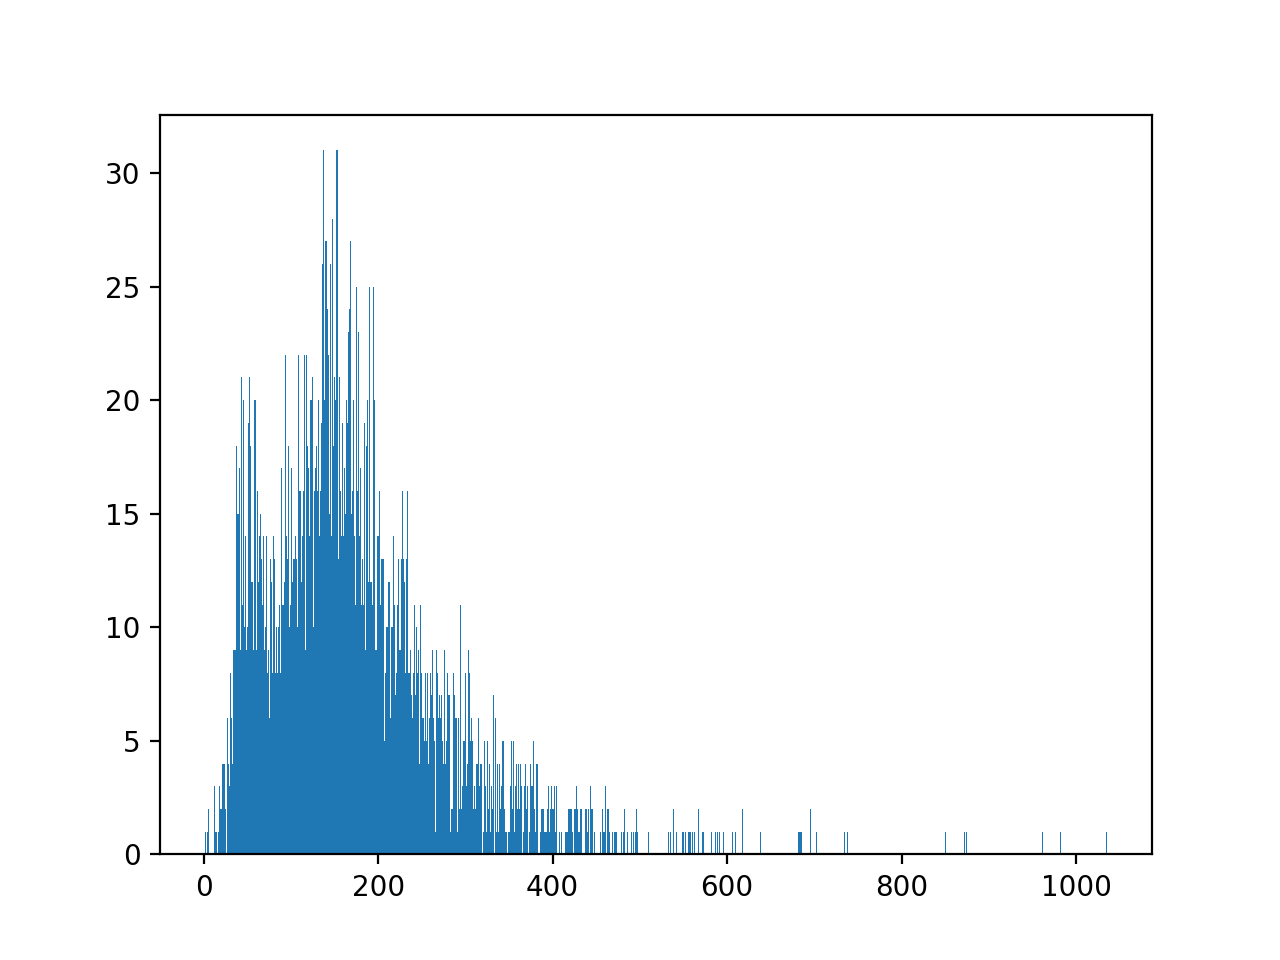
\includegraphics[scale=0.5]{lengthD}\\
	\textbf{Figure 5. Essay Length Distribution (CAES)}
	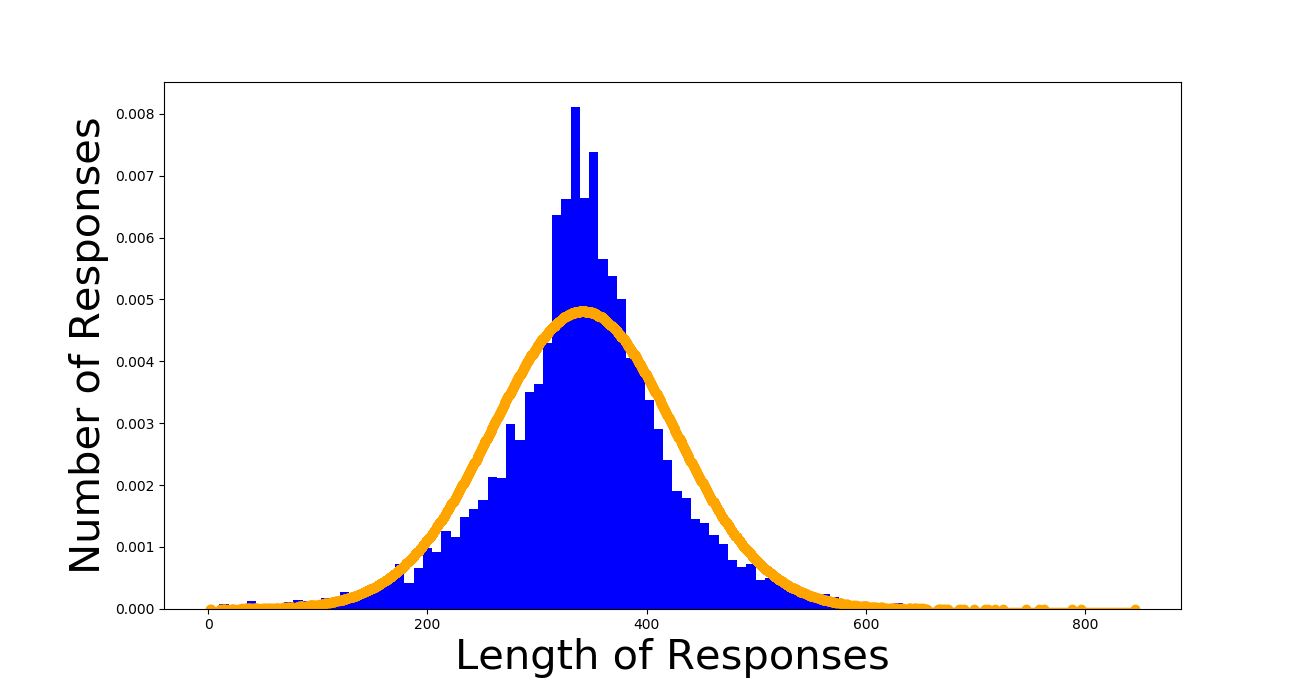
\includegraphics[scale=0.25]{Figure1}\\
	\textbf{Figure 6. Essay Length Distribution (TOEFL)}
\end{center}


\section{Methods}
\subsection{Tools, Libraries, and Software}
Outlined below are all the relevant electronic resources that were used to carry out our experiments. External resources (such as models or classifiers) are outlined in later sections.\\
\\
$\bullet$ Hardware: Windows 10 (custom-build) 4.20 GHz Intel Core i5-7600K. GTX 1070 GPU.\\
$\bullet$ Software: Python 3.5\\
$\bullet$ Libraries: Tensorflow, numpy, sklearn\\
$\bullet$ Development Tools: Git, Slack\\
\\
Using slack as out main channel of communication, our group was able to outline project goals and directives, and informally collaborate on code. Git was used for overall development to push and pull new additions to the NLI Project. Python 3.5 was the language of choice, and specifically the tensorflow, numpy, and sklearn libraries were used to preprocess the information into vectors and use NNs as classifiers. All of this was carried out on an XPS 13 machine (windows environment).
\subsection{External Resources}
\tab As mentioned in the Introduction, the main classifiers that were used were a Recurrent Neural Net and a Convolutional Neural Net. We were able to use tensorflow to create these nets. Each net had 3 hidden layers with 10000 vector embeddings and utilized a ReLU activation function.
\subsection{Experiments}
\tab Our experiments involved using two different neural nets and four (total) different optimizers to create a system that had the highest accuracy for NLI classification. These classifiers and optimizers are outlined below:\\
\\
\textbf{Convolutional Neural Net with:}\\
\tab $\bullet$ ``Adam" Optimizer\\
\tab $\bullet$ ``Adam" Optimizer and trigrams\\
\tab $\bullet$ rms propogation\\
\\
\textbf{Recurrent Neural Net with:}\\
\tab $\bullet$ ``Adam" Optimizer\\
\tab $\bullet$ ``Adam" Optimizer and trigrams\\
\tab $\bullet$ Dynamic ``Adam" Optimizer\\
\\
More information on optimizers is outlined in the following section:
\subsubsection*{Background Information on Optimizers}
\tab When deciding which class of optimizers to use for the machine learning optimization, it seemed that there was no perfect “scenario” that described when to use each stochastic gradient descent algorithm. Throughout the ML community it seems that the “right” algorithm to use can depend largely on the amount of available computer power (mobile device or laptop vs. supercomputer or grid), size of the data, type of the optimization problem (convex, non convex, etc.), or many other factors unique to each model. While changing the parameters of algorithms in certain ways works well with some optimizers (and poorly for others), because we chose to use three of the best rated algorithms, their differences in performance likely won't be (and ultimately were not) drastically different.\\
\tab RMSProp (Root Mean Square Propogation) maintains a moving average of the square of gradients and is most commonly used to resolve Adagrad’s radically diminished learning rates. While we did not use Adagrad, RMSprop also divides the learning rate by an exponentially decaying average in order to make the data the model was originally trained on have more weight than data introduced later. This algorithm has shown to be useful for noisy problems and iteratively adapts to the training data. The Adam optimizer is another method that computes adaptive learning rates and is similar to RMSProp in how it keeps an exponentially decaying average of past gradients. We chose to experiment with this over the Momentum optimizer, because while the Momentum optimizer behaves like a ball running down a slope, the Adam optimizer behaves like a ball with more friction and therefore prefers a flat minimum in the error surface. The Adam optimizer is recommended in the field of deep learning because it attains high accuracy relatively quickly compared to other optimizers, and this was helpful as we trained our models on laptops with limited computing power. \\ \tab Adam also incorporates the benefits of AdaGrad and RMSProp. Instead of adapting the parameter learning rates based on the average first moment (the mean) as in RMSProp, Adam also makes use of the average of the second moments of the gradients (the uncentered variance). Ultimately while we did not observe a dramatic difference between these optimizers, with a larger and more diverse dataset it is possible that one would have performed significantly better than others.

\section{Results}
\subsection{Data Partitioning}
As mentioned earlier, for the CAES dataset 90\% of the essays were devoted towards training, whereas 10\% were held in reserve. It should be noted that the 90\% and 10\% were selected at random by shuffling the entire dataset with the random library in python. The TOEFL dataset was partitioned in the same way.
\subsection{Accuracy \& Loss}
Please see \textbf{Figure 7}, \textbf{Figure 8}, \textbf{Figure 9} and \textbf{Figure 10} below for loss and accuracy results for the CAES datasets. These are determined by classifier/optimizer and by epochs completed. Note that our group was using a random baseline of 16.6\% for the CAES data (6 languages total, so 1/6 chance of guessing correctly) and 9.99\% baseline for the TOEFL tags (11 languages total, 1/11 chance of guessing correctly). \\
\begin{center}
	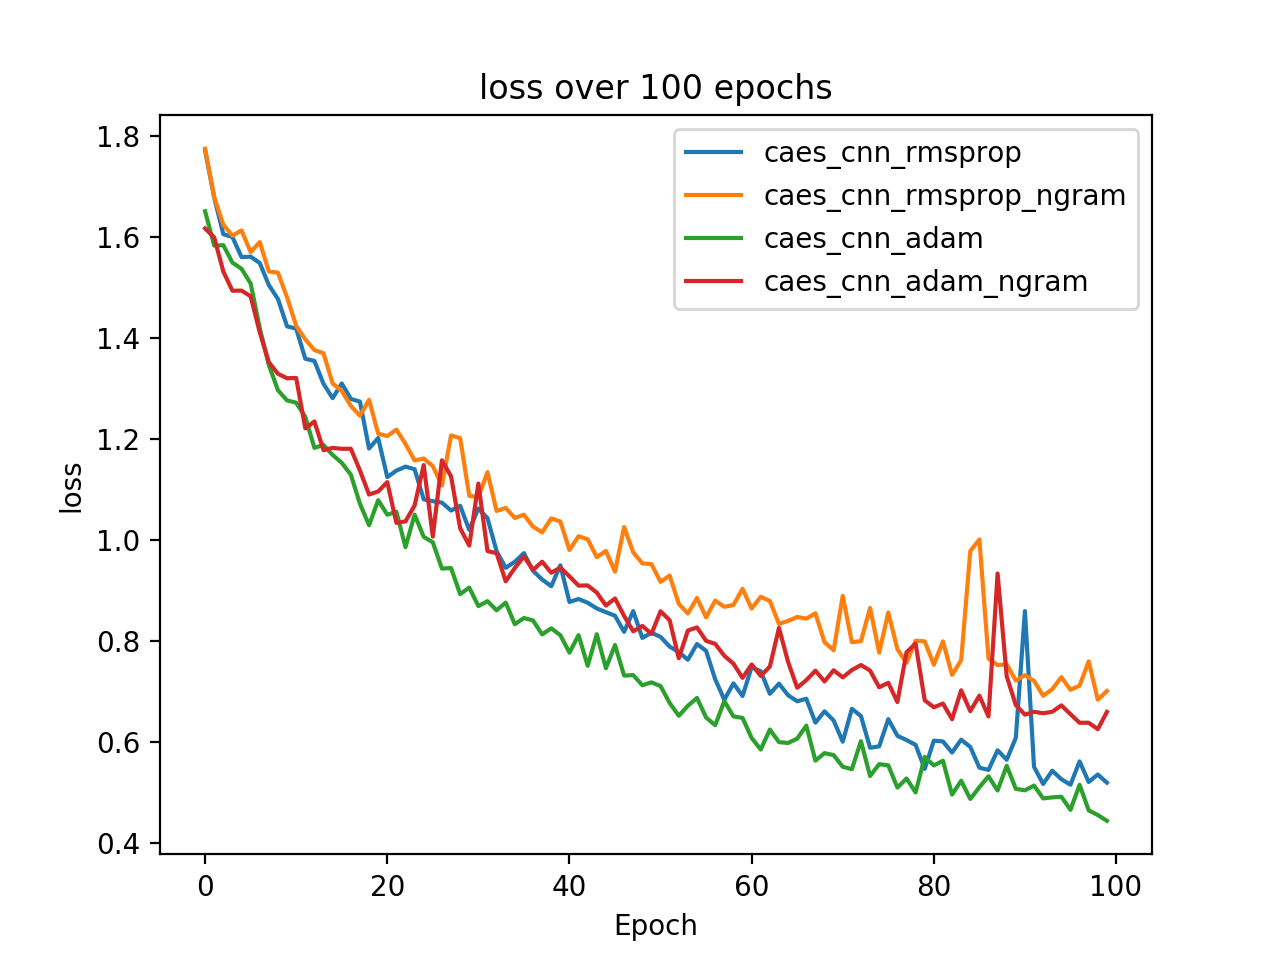
\includegraphics[scale=0.5]{lo1}\\
	\small \textbf{Figure 7. Loss per Epoch (CAES)}
	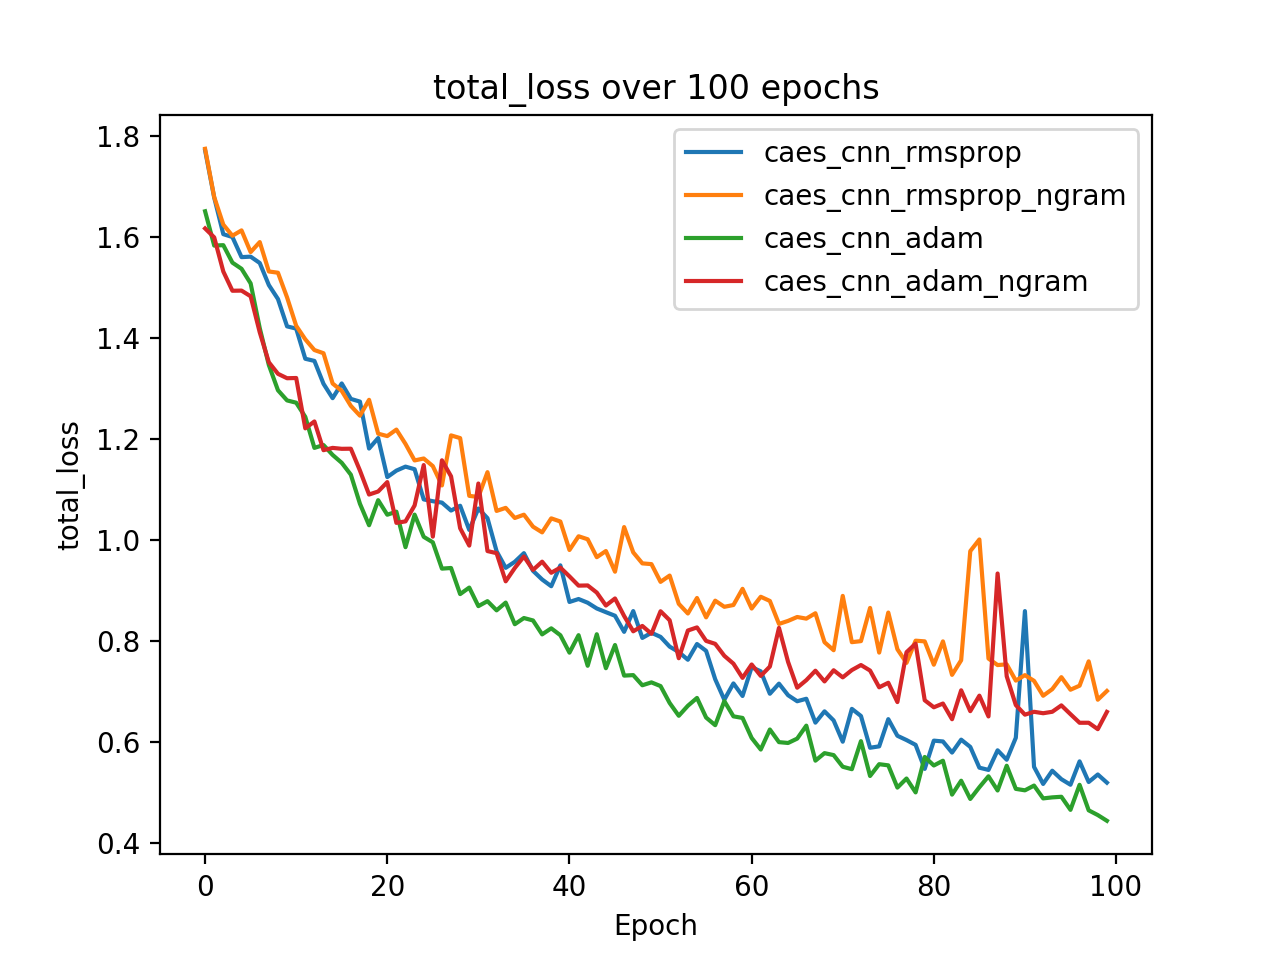
\includegraphics[scale=0.5]{tl01}\\
	\small \textbf{Figure 8. Total Loss (CAES)}
	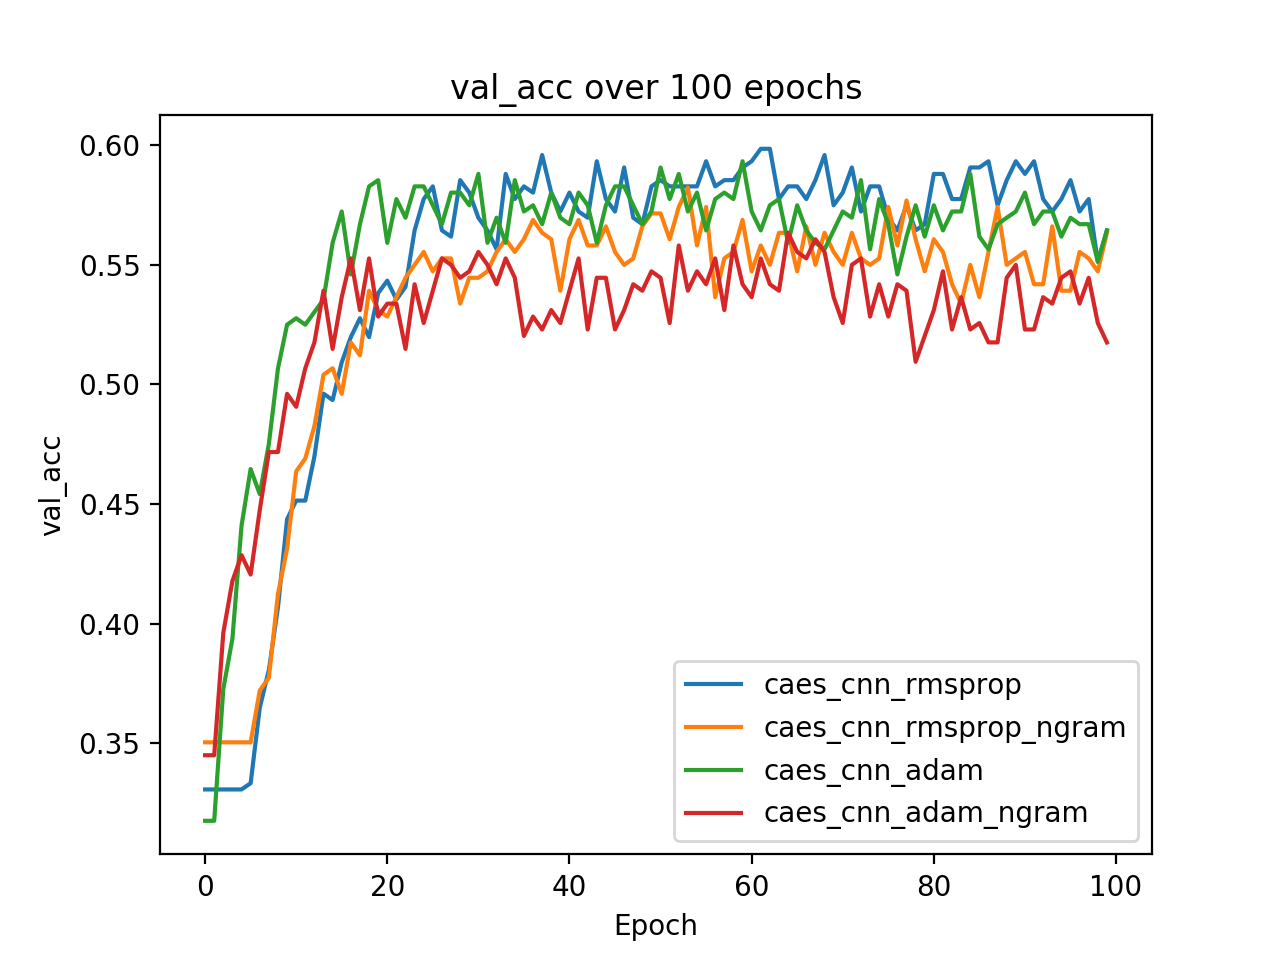
\includegraphics[scale=0.5]{vall}\\
	\small \textbf{Figure 9. Classifier Accuracy (Training Set, CAES)}
	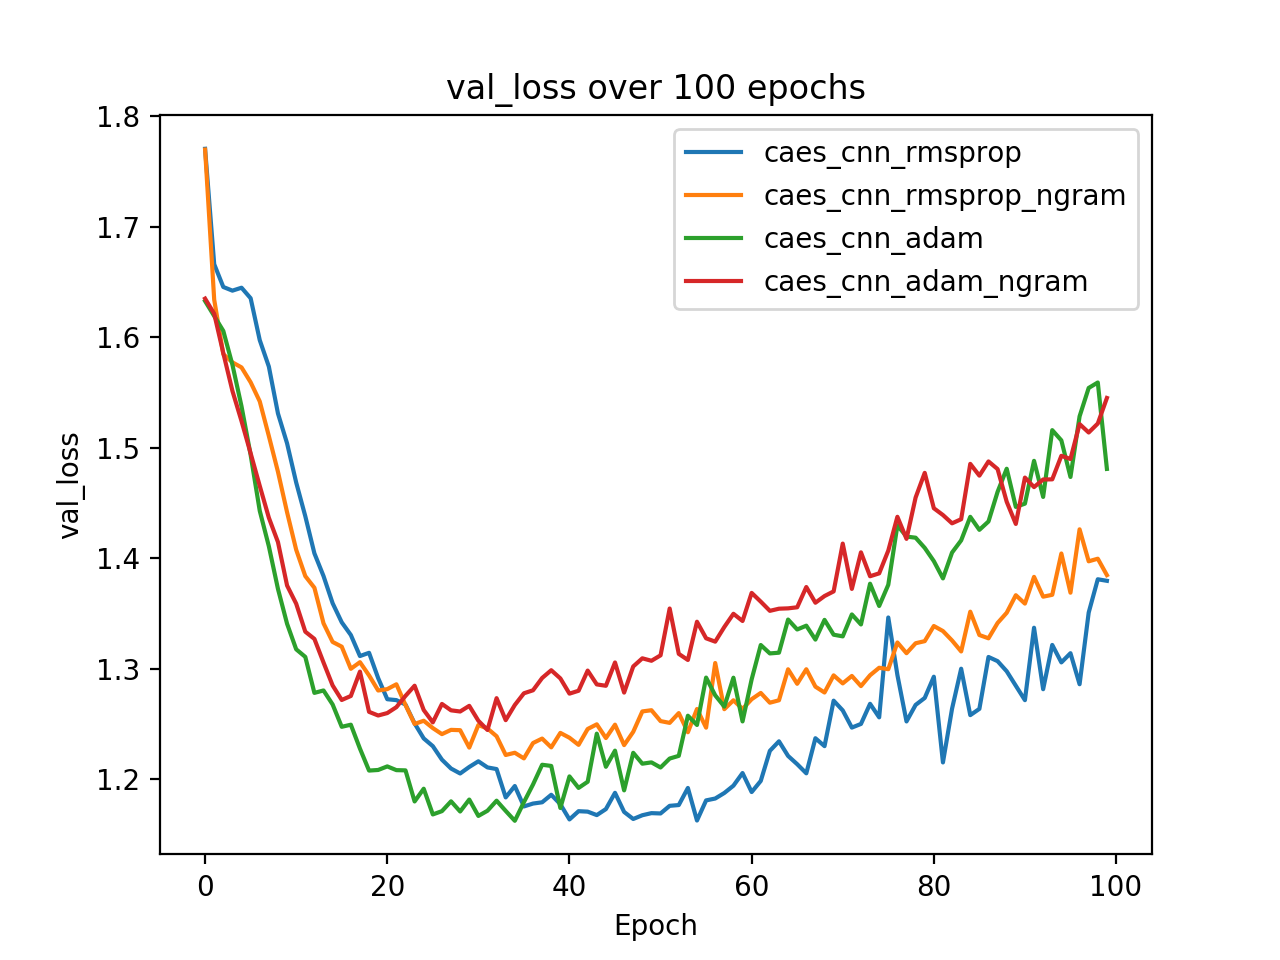
\includegraphics[scale=0.5]{vlo}\\
	\small\textbf{Figure 10. Classifier Accuracy (Test Set, CAES) }
\end{center}
\tab As we can see from the above graphs, all the classifiers have nearly the same accuracy (hovering around 50\% by the time they hit the 100th epoch). Surprisingly, two of the CNNs were among the most accurate classifiers. Specifically, the CNN with ``adamn" optimizer and trigrams had the highest accuracy, peaking around 53\% and stabilizing around 46\%. The CNN with RMS propogation also performed well (around 45\%). Amongst the RNNs, the RNN just utilizing the ``adam" optimizer performed well, ending a around 46\%. Note that from the loss function graph, the CNN with ``adamn" optimizer and trigrams had the lowest loss, totaling around 0.8. However, the RNN with ``adam" and trigrams was also around this value too. Our classifiers in all instances beat our random baseline, which is encouraging. However, not a single one was able to correctly guess the native language (consistently) more than 50\% of the time. This could be improved upon. \textbf{NOTE: Results regarding the classifier accuracy on the TOEFL dataset will be included in the final draft.}
\section{Conclusions \& Future Work}
\tab Although we achieved our goal of creating a system that could guess a person’s native language correctly more than 16.6\% of the time (which is better than randomly guessing), there is still opportunity for our model to increase its accuracy. Our highest performing classifier obtained an accuracy of about 50\%. While we believe that this is a great start, we think that continuing to tweak the parameters in our classifiers, optimizers, and neural net still has the potential to yield better results. If we were to do this project again, an opportunity for growth could have arisen from using different corpuses that consist of more essays and a larger distribution of native languages. While the TOEFL corpus we utilized offered 11 languages, by increasing this number to more than 30 languages and incorporating a larger number of essays for each language, we believe that the model would be better able to accurately guess a writer’s native language. Further experimentation could also include utilizing native classifiers like SVM and doing further research on the unique differences of different stochastic gradient descent algorithms.\\
\tab Ultimately this project was a great opportunity to learn the basics of TensorFlow, create neural networks, train models, implement different optimization algorithms, and analyze the data to determine how subtle differences in parameters and values can have a drastic effect on the network. Moving forward we hope to continue to enhance the inference ability of our model and eventually be able to identify not just 5, but several additional languages written by people of a diverse range of language and writing abilities.

%\section*{References}
% include your own bib file like this:
%\bibliographystyle{acl_natbib}
%\bibliography{acl2018}
%\bibliography{acl2018}
%fs\bibliographystyle{acl_natbib}
\end{document}
